\documentclass[aspectratio=169]{beamer}
\usepackage[utf8]{inputenc} % codificacao de caracteres
\usepackage[T1]{fontenc}    % codificacao de fontes
\usepackage[english]{babel}  % idioma
\usepackage{graphics,amssymb,amsfonts,amsmath,xfrac}
\usepackage{tikz}
\usepackage{enumerate,hyperref}
\usepackage{palatino}	% Fonte sem serifa
\usepackage{ragged2e}	% Paragrafo justificado
%\usepackage{minted}	% Highlight para codigos de programacao
\usepackage{booktabs} % tabelas
\usepackage{multicol}
\usepackage{multirow}
\usepackage{mathrsfs}
\usepackage{relsize}

%\usepackage[table]{xcolor}
\newcommand{\Laplace}[1]{\ensuremath{\mathcal{L}{\left[#1\right]}}}
\newcommand{\InvLap}[1]{\ensuremath{\mathcal{L}^{-1}{\left[#1\right]}}}

% Veja mais temas e cores em http://www.hartwork.org/beamer-theme-matrix/
\usetheme{Montpellier}         % tema
\usecolortheme{orchid}      % cores
\usefonttheme[onlymath]{serif} % fonte modo matematico
% Colocando numero de paginas no slide
\setbeamertemplate{footline}[frame number]



\DeclareGraphicsExtensions{.pdf,.JPG,.png} % compilamos apenas com pdflatex
%\graphicspath{{./figuras/}} % caminho onde as figuras estarao disponiveis


\graphicspath{{figuras/}}

% ---------------------------------------------------------------------------- %
% T�tulo                                                                       %
% ---------------------------------------------------------------------------- %

\title[\sc{Teoria de Circuitos Eletrônicos 1}]{\LARGE Aula 12 - The Laplace
Transform}
\author[Prof. Marcelino Andrade]{Prof. Marcelino Andrade}
\institute{Faculdade UnB Gama} % opcional
\date{\today}

\begin{document}
\justifying % Paragrafo justificado
\pagebreak

\begin{frame}
  \titlepage
\end{frame}


% ----------------- NOVO SLIDE --------------------------------
\begin{frame}{Contents}

\tableofcontents
%\begin{center}	
     		Introduction to Electric Circuits by James A. Svoboda, Richard C. Dorf, 9th Edition 
  %   		Fundamentals of Electric Circuits by Alexander and Sadiku, 4th Edition	
%\end{center}	
\end{frame}

% ----------------- NOVA SECÇÂO -----------------------------
\section{Introduction (14.1)}
% ----------------- NOVO SLIDE --------------------------------
\begin{frame}[fragile]
	\frametitle{Introduction}
		\begin{tabular}{cc}
			\begin{columns}
				\begin{column}{1\textwidth}  %%<--- here
The Laplace transform is a very powerful tool for the analysis of circuits and enables the circuit analyst to transform the set of differential equations describing a circuit
to the complex frequency domain, where they become a set of linear algebraic equations. In this chapter,	
		
\small		\begin{itemize}
						\item[$\clubsuit$]{We find the complete response;\newline}
						\item[$\clubsuit$]{We analyzed transient part plus steady-state part;\newline}
						\item[$\clubsuit$]{We analyzed first-order and second-order circuits;\newline}		
						\item[$\clubsuit$]{we analyzed stability of the circuits.\newline}	
					\end{itemize}
					
				\end{column}
			\end{columns}
		
	\end{tabular}
\end{frame}

% ----------------- NOVA SECÇÂO -----------------------------
\section{Laplace Transform (14.2)}
% ----------------- NOVO SLIDE --------------------------------
\begin{frame}[fragile]
	\frametitle{Direct and inverse Laplace transform }
		\begin{tabular}{cc}
		\begin{columns}
		\begin{column}{1\textwidth}  %%<--- here

	The $\mathscr{L}\{f(t)\}$  indicates taking the Laplace transform of $f(t)$. The result, $F(s)$,
is called the Laplace transform of $f(t)$.  \newline	

				\end{column}
				\end{columns}\\
	\begin{columns}
	\begin{column}{.5\textwidth}  %%<--- here
The (one-sided or unilateral) \textbf{Laplace transform} is defined as
\begin{center}		$F(s)=\mathscr{L}\{f(t)\}=\int_{0}^{\infty}\!f(t)e^{-st}\mathrm{d}t$ \end{center}

 
				\end{column}
\begin{column}{.5\textwidth}  %%<--- here\
The \textbf{inverse Laplace transform} is defined by the complex inversion integral
\begin{center}		$f(t)=\mathscr{L}^{-1}\{F(s)\}=\frac{1}{2 \pi j}\int_{\alpha-j\infty}^{\alpha+\infty}\!F(s)e^{st}\mathrm{d}s$ \end{center}
 
 
				\end{column}				
	\end{columns}\\	
		\begin{columns}
		\begin{column}{1\textwidth}  %%<--- here
\newline \newline	Where $s$ is a complex variable given $s=\sigma+j\omega$.  		The function $f(t)$ is said to exist in the time domain,
where as the function $F(s)$ is said to exist in the  $s$-domain.

				\end{column}
				\end{columns}\\				
			
				
				
				
	\end{tabular}		
\end{frame}


% ----------------- NOVO SLIDE --------------------------------
\begin{frame}[fragile]
	\frametitle{Direct and inverse Laplace transform}
\begin{tabular}{ll}
	\begin{columns}
		\begin{column}{1\textwidth}  %%<--- here
We say that $f(t)$ and $F(s)$ comprise a Laplace transform pair and denote this fact as 
\begin{center} $f(t) \Leftrightarrow F(s)$ \end{center} 		
		\end{column}
	\end{columns}\\
	\begin{columns}
		\begin{column}{0.5\textwidth}  %%<--- here	
		\begin{center}
		The transform method is summarized in Figure Below. \newline
    			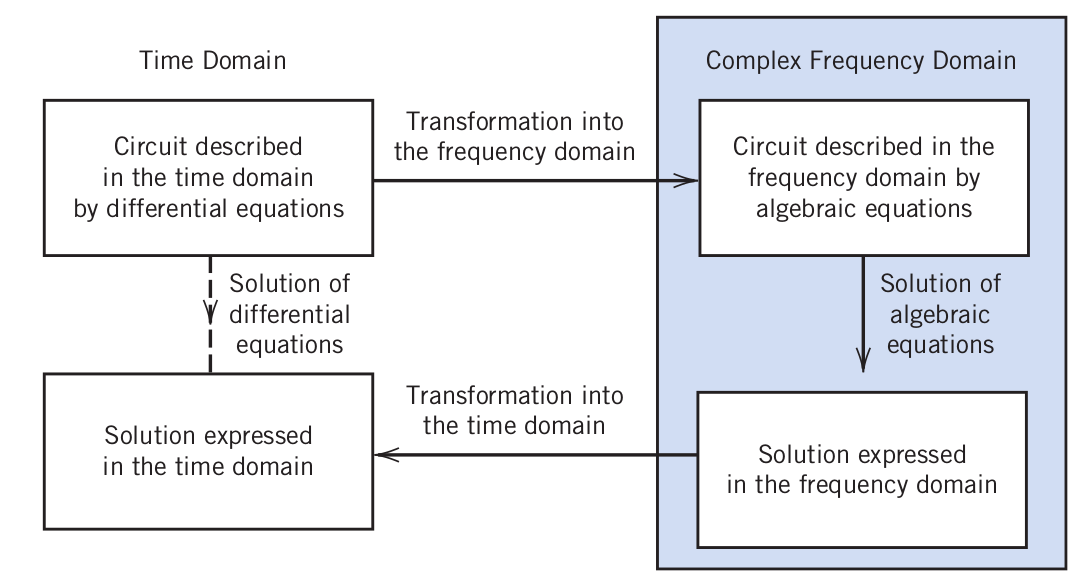
\includegraphics[height=3.5cm]{figure1.png}	
		\end{center}	
		\end{column}
		\begin{column}{0.5\textwidth}  %%<--- here	
		\textbf{EXERCISE 14.2-1} - Laplace Transform Pairs. \newline \\
%		\begin{center}
(a) Find the Laplace transform of $f(t)=e^{-at}$, where $a > 0$. \newline
(b) Find the Laplace transform of $f(t)=e^{-at}u(t)$, where $a > 0$ and $u(t)$ is the unit step function.	
%		\end{center}	
		\end{column}
	\end{columns}
	\end{tabular}
\end{frame}

% ----------------- NOVO SLIDE --------------------------------
\begin{frame}[fragile]
	\frametitle{Linearity}
\begin{tabular}{ll}
	\begin{columns}
		\begin{column}{1\textwidth}  %%<--- here
Linearity is an important property of the Laplace transform. 
\begin{center} $a_1f_1(t)+a_2f_2(t) \Leftrightarrow a_1F_1(s)+a_2F_2(s)$ \end{center}   
\begin{center} {} \end{center} 
		\end{column}
	\end{columns}\\
	\begin{columns}
		\begin{column}{0.5\textwidth}  %%<--- here	
\small We have \newline
		
		$F(s)=\mathscr{L}\{f(t)\}$\\
		$F(s)=\mathscr{L}\{a_1f_1(t)+a_2f_2(t)\}$
		$F(s)=\mathscr{L}\{a_1f_1(t)\}+\mathscr{L}\{a_2f_2(t)\}$\\
		$F(s)=a_1\mathscr{L}\{f_1(t)\}+a_2\mathscr{L}\{f_2(t)\}$\\
		$F(s)=a_1F_1(s)+a_2F_2(s)$\\

		
		\end{column}
		\begin{column}{0.5\textwidth}  %%<--- here	
\small		Where $F_1(s)$ and $F_2(s)$ are the Laplace transforms of the time functions $f_1(t)$ and $f_2(t)$, respectively.\newline\\
		\textbf{EXERCISE 14.2-2} - Linearity. \newline \\
%		\begin{center}
Find the Laplace transform of $\sin (\omega t)$.	
%		\end{center}	
		\end{column}
	\end{columns}
	\end{tabular}
\end{frame}
% ----------------- NOVO SLIDE --------------------------------
\begin{frame}[fragile]
	\frametitle{Differentiation in the Time Domain}
\begin{tabular}{ll}
	\begin{columns}
		\begin{column}{1\textwidth}  %%<--- here
We can summarize differentiation in the time domain as 
\begin{center} $\frac{df}{dt} \Leftrightarrow sF(s)-f(0^{-1})$ \end{center}   
\begin{center} {} \end{center} 
		\end{column}
	\end{columns}\\
	\begin{columns}
		\begin{column}{0.5\textwidth}  %%<--- here	
\small We have \newline
		
		$\mathscr{L}\{\frac{\mathrm{d}f}{\mathrm{d}t}\}=\int_{0}^{\infty}\!\frac{\mathrm{d}f}{\mathrm{d}t}e^{-st}\mathrm{d}t$ \newline \\
		Integrating by parts \newline \\
		$\mathscr{L}\{\frac{\mathrm{d}f}{\mathrm{d}t}\}=s \int_{0}^{\infty} \ fe^{-st}\mathrm{d}t + fe^{-st}\Big|_{0}^{\infty} $ \\
		$\mathscr{L}\{\frac{\mathrm{d}f}{\mathrm{d}t}\}=sF(s)-f(0^{-1})$ \\


		
		\end{column}
		\begin{column}{0.5\textwidth}  %%<--- here
\small		Thus, the Laplace transform of the derivative of a function is s times the Laplace transform of the
function minus the initial condition. \newline \\
		\textbf{EXERCISE 14.2-3} - Differentiation in the Time Domain. \newline \\
%		\begin{center}
Find the Laplace transform of $\cos (\omega t)$.	
%		\end{center}	
		\end{column}
	\end{columns}
	\end{tabular}
\end{frame}




% ----------------- NOVO SLIDE --------------------------------
\begin{frame}[fragile]
	\frametitle{Direct and inverse Laplace transform}
\begin{tabular}{ll}

	\begin{columns}
		\begin{column}{0.5\textwidth}  %%<--- here
Thus, we use the definition of the Laplace transform to obtain
Laplace transform pairs. \newline \\ Table provides a
collection of important Laplace transform pairs. 
		\end{column}
		\begin{column}{0.5\textwidth}  %%<--- here
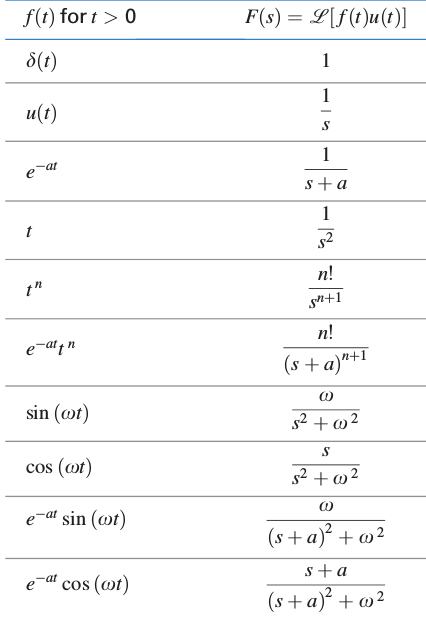
\includegraphics[height=6.5cm]{figure2.png}

		\end{column}
	\end{columns}\\	
\end{tabular}
\end{frame}
% ----------------- NOVO SLIDE --------------------------------
\begin{frame}[fragile]
	\frametitle{Direct and inverse Laplace transform}
\begin{tabular}{ll}

	\begin{columns}
		\begin{column}{0.3\textwidth}  %%<--- here
Thus, we use the definition of the Laplace transform to obtain
properties of the Laplace transform. \newline \\ Table lists important properties of the Laplace
transform.
		\end{column}
		\begin{column}{0.7\textwidth}  %%<--- here
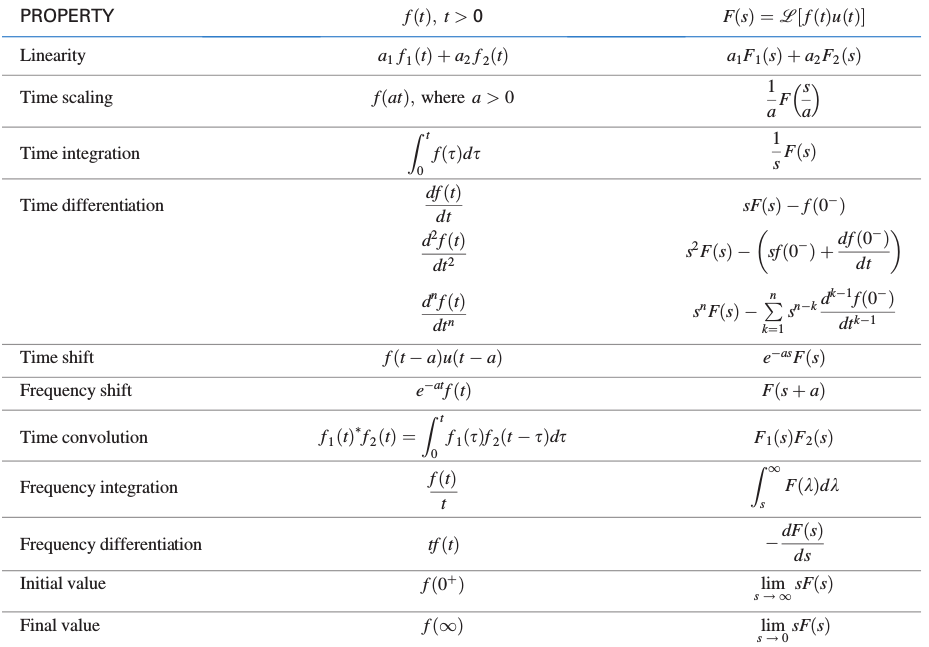
\includegraphics[height=6.5cm]{figure3.png}

		\end{column}
	\end{columns}\\	
\end{tabular}
\end{frame}
% ----------------- NOVO SLIDE --------------------------------
\begin{frame}[fragile]
	\frametitle{Laplace Transform}
\begin{tabular}{ll}
	\begin{columns}
		\begin{column}{1\textwidth}  %%<--- here
\newline \newline		\textbf{EXERCISE 14.2-4} - Find the Laplace transform of $5-5e^{-2t}(1+2t)$.\\
		\scalebox{0.8}{Answer: $\dfrac{20}{s(s^2+4s+4)}$}
		\end{column}
	\end{columns}\\
	\begin{columns}
		\begin{column}{1\textwidth}  %%<--- here
\newline \newline		\textbf{EXERCISE 14.2-5} - Find the Laplace transform of $10e^{-4t}cos(20t+36.9^o)$.\\
		\scalebox{0.8}{Answer: $\dfrac{8s-88}{s^2+8s+416}$}
		\end{column}
	\end{columns}\\
	\begin{columns}
		\begin{column}{1\textwidth}  %%<--- here
\newline \newline		\textbf{EXERCISE 14.2-6} - Find the Laplace transform of $2 \delta(t) +3 + 4u(t)$.\\
		\scalebox{0.8}{Answer: $2 + \dfrac{7}{s}$}
		\end{column}
	\end{columns}\\
\end{tabular}
\end{frame}

% ----------------- NOVA SECÇÂO -----------------------------

\section{Pulse Inputs (14.3)}
% ----------------- NOVO SLIDE --------------------------------
\begin{frame}[fragile]
	\frametitle{Pulse Inputs}
\begin{tabular}{ll}

	\begin{columns}
		\begin{column}{0.5\textwidth}  %%<--- here
The step function is represented as
$$
	    u(t)=
	    \begin{cases}
	    0, \ when \ t < 0 \\
	    1, \ when \ t > 1 \\
	    
	    \end{cases}
	    $$
makes an abrupt transition from 0 to 1 at time $t=0$. 
Define the impulse function $\delta (t)$ to be
$$
	    \delta (t)= \dfrac{d}{dt}u(t)
	    \begin{cases}
	    0, \ when \ t < 0 \\
	    undefined, \ when \ t = 0 \\
	    0, \ when \ t > 0 \\	    
	    \end{cases}
	    $$

		\end{column}
		\begin{column}{0.5\textwidth}  %%<--- here
Because $\delta(t)$ is undefined at time 0, we consider the function $u_{\varepsilon}(t)$. This
function makes the transition from 0 to 1 over the time interval from 0 to $\varepsilon$. Notice that
$$\lim_{\varepsilon \to 0} u_{\varepsilon}(t)=u(t)$$

$$
	    \delta_{\varepsilon} (t)= \dfrac{d}{dt}u_{\varepsilon}(t)
	    \begin{cases}
	    0, \ when \ t < 0 \\
	    \dfrac{1}{\varepsilon}, \ when \ 0 < t < \varepsilon \\
	    0, \ when \ t > \varepsilon\\	    
	    \end{cases}
	    $$

		\end{column}
	\end{columns}\\	
\end{tabular}
\end{frame}
% ----------------- NOVO SLIDE --------------------------------
\begin{frame}[fragile]
	\frametitle{Pulse Inputs}
\begin{tabular}{ll}

	\begin{columns}
		\begin{column}{0.25\textwidth}  %%<--- here
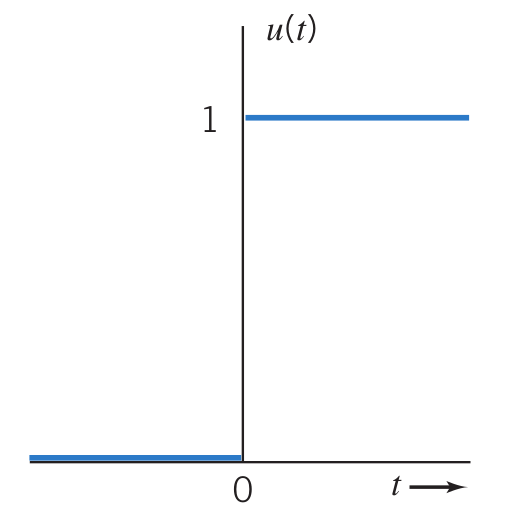
\includegraphics[height=3.5cm]{figure4.png}

		\end{column}
		\begin{column}{0.25\textwidth}  %%<--- here
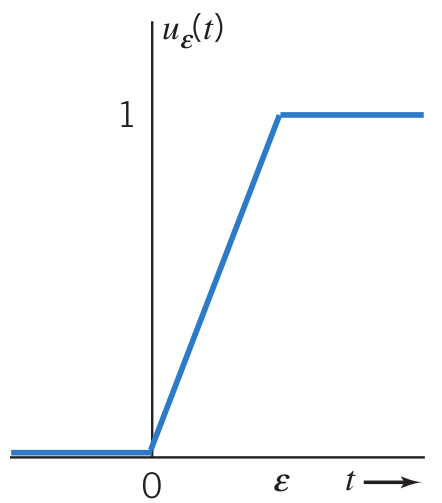
\includegraphics[height=3.5cm]{figure5.png}

		\end{column}
		\begin{column}{0.25\textwidth}  %%<--- here
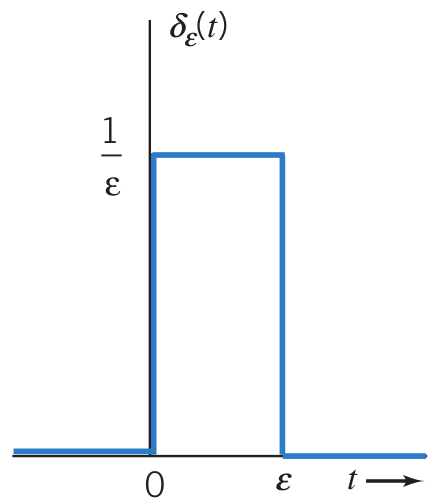
\includegraphics[height=3.5cm]{figure6.png}

		\end{column}
		\begin{column}{0.25\textwidth}  %%<--- here
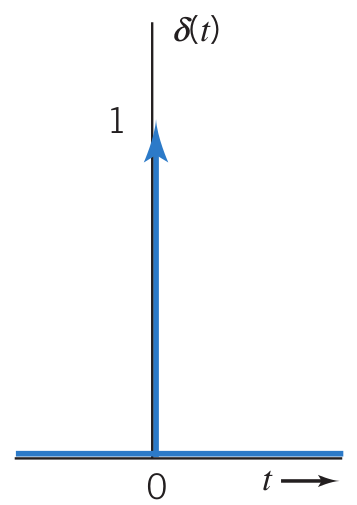
\includegraphics[height=3.5cm]{figure7.png}

		\end{column}		
	\end{columns}\\	
	\begin{columns}
		\begin{column}{0.25\textwidth}  %%<--- here
$$u(t)=\lim_{\varepsilon \to 0} u_{\varepsilon}(t)$$

		\end{column}
		\begin{column}{0.25\textwidth}  %%<--- here
\tiny $$
	    u_{\varepsilon} (t)=
	    \begin{cases}
	    0, \ when \ t < 0 \\
	    \dfrac{1}{\varepsilon}t, \ when \ 0 < t < \varepsilon \\
	    1, \ when \ t > \varepsilon\\	    
	    \end{cases}
	    $$

		\end{column}
		\begin{column}{0.25\textwidth}  %%<--- here
\tiny $$
	    \delta_{\varepsilon} (t)=
	    \begin{cases}
	    0, \ when \ t < 0 \\
	    \dfrac{1}{\varepsilon}, \ when \ 0 < t < \varepsilon \\
	    0, \ when \ t > \varepsilon\\	    
	    \end{cases}
	    $$

		\end{column}
		\begin{column}{0.25\textwidth}  %%<--- here
$$\delta(t)=\lim_{\varepsilon \to 0} \delta_{\varepsilon}(t)$$

		\end{column}		
	\end{columns}\\		
	
	
	
\end{tabular}
\end{frame}
% ----------------- NOVO SLIDE --------------------------------
\begin{frame}[fragile]
	\frametitle{Pulse Inputs}
\begin{tabular}{ll}

	\begin{columns}
		\begin{column}{0.5\textwidth}  %%<--- here
\small Notice that for any value of $\varepsilon$, the area
under the pulse is given by
\small $$\int_{-\infty}^{+\infty}\! \delta_{\varepsilon} (t)\ \mathrm{d}t=\int_{0}^{\varepsilon}\! \dfrac{1}{{\varepsilon}} t \ \mathrm{d}t=1$$
\\
\small An important property of the impulse function is
\small $$
\int_{-\infty}^{+\infty}\! f(t)\delta(t) \mathrm{d}t=f(0)   $$
\small Letting $f(t)=1$ gives
\small $$
\int_{-\infty}^{+\infty}\! \delta(t) \mathrm{d}t=1   $$

		\end{column}
		\begin{column}{0.5\textwidth}  %%<--- here
\small  \textbf{EXERCISE 14.3-1} - Find the Laplace transform of $f(t)$, $g(t)$ and, $h(t)$ shown in Figure below.\\
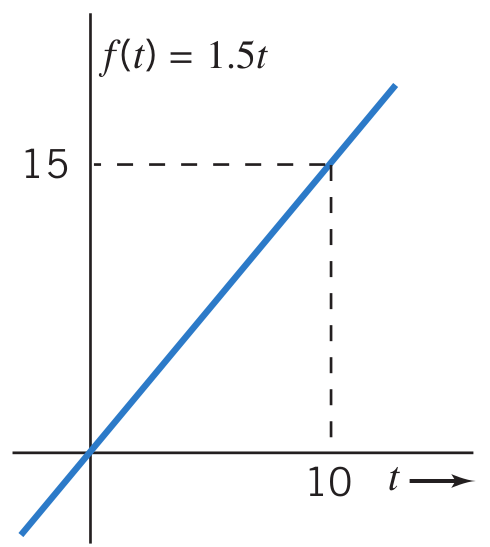
\includegraphics[height=2.5cm]{figure8.png}
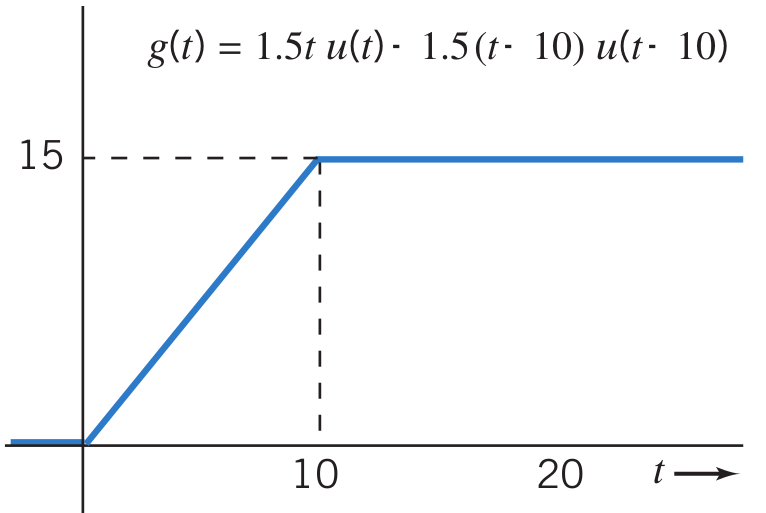
\includegraphics[height=2.5cm]{figure9.png}\\
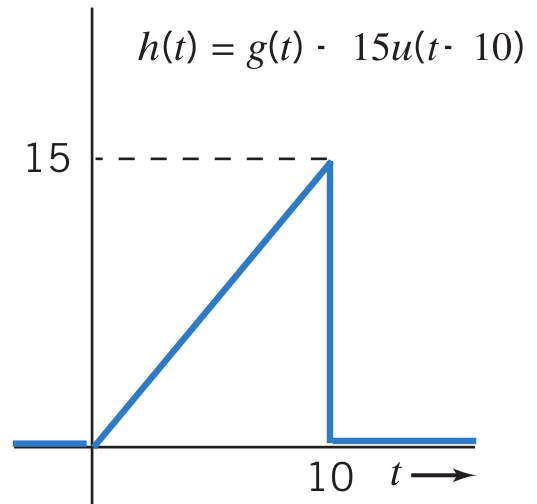
\includegraphics[height=2.5cm]{figure10.png}\\
		\end{column}
	\end{columns}\\	
\end{tabular}
\end{frame}


% ----------------- NOVA SECÇÂO -----------------------------
\section{Inverse Laplace Transform (14.4)}
% ----------------- NOVO SLIDE --------------------------------
\begin{frame}[fragile]
	\frametitle{Inverse Laplace }
\begin{tabular}{ll}

	\begin{columns}
	\small	\begin{column}{1\textwidth}  %%<--- here
We will frequently want to find the inverse Laplace transform of a function represented as a ratio of
polynomials in $s$. Consider:

$$F(s)=\dfrac{N(s)}{D(s)}=\dfrac{b_ms^m+b_{m-1}s^{m-1}+...+b_{1}s+b_{0}}{s^n+a_{n-1}s^{n-1}+...+a_{1}s+a_{0}} $$

The roots of the denominator polynomial $D(s)$ are the roots of the equation $D(s)=0$ and are
called the poles of $F(s)$. Factoring $D(s)$, we obtain
$$F(s)=\dfrac{N(s)}{D(s)}=\dfrac{b_ms^m+b_{m-1}s^{m-1}+...+b_{1}s+b_{0}}{(s-p_1)(s-p_2)...(s-p_n)} $$
The roots of the numerator polynomial $N(s)$ are
called the zeros of $F(s)$.

		\end{column}

	
	\end{columns}\\


\end{tabular}	
\end{frame}
% ----------------- NOVO SLIDE --------------------------------
\begin{frame}[fragile]
	\frametitle{Inverse Laplace }
\begin{tabular}{ll}

	\begin{columns}
	\small	\begin{column}{1\textwidth}  %%<--- here

	We will find the inverse Laplace transform of a proper rational function $F(s)$ in three steps.
	
	
	\small		\begin{enumerate}
\item{First, we perform a partial fraction expansion to express $F(s)$ as a sum of simpler functions, $F_i(s)$;}
$$ F(s)=F_1(s)+F_2(s)+...+F_i(s)+...+F_n(s)$$
\item{Next, we use the transform pairs and properties to find the inverse
Laplace transform of each $F_i(s)$;\newline}
\item{Finally, using linearity, we sum the inverse transforms of the $F_i(s)$ to
obtain the inverse Laplace transform of $F(s)$;\newline}			
					\end{enumerate}
					

		\end{column}

	
	\end{columns}\\


\end{tabular}	
\end{frame}
% ----------------- NOVO SLIDE --------------------------------
\begin{frame}[fragile]
	\frametitle{Simple Poles }
\begin{tabular}{ll}

	\begin{columns}
	\small	\begin{column}{1\textwidth}  %%<--- here

	When all of the poles of a proper rational function, $F(s)$, are simple poles, the partial fraction
expansion of $F(s)$ is
	$$F(s)=\dfrac{N(s)}{D(s)}=\dfrac{b_ms^m+b_{m-1}s^{m-1}+...+b_{1}s+b_{0}}{s^n+a_{n-1}s^{n-1}+...+a_{1}s+a_{0}} $$
	$$F(s)=\dfrac{R_1}{s-p_1}+\dfrac{R_2}{s-p_2}+...+\dfrac{R_i}{s-p_i}+...+\dfrac{R_n}{s-p_n} $$
	The coefficients $R_i$ are called residues.The values of the residues of simple poles are calulated as	
	$$R_i=(s-p_i)F(s) \big |_{s=p_i}$$

					

		\end{column}

	
	\end{columns}\\


\end{tabular}	
\end{frame}
% ----------------- NOVO SLIDE --------------------------------
\begin{frame}[fragile]
	\frametitle{Complex Conjugate Poles}
\begin{tabular}{ll}

	\begin{columns}
	\small	\begin{column}{1\textwidth}  %%<--- here

	Suppose $F(s)$ has a pair of simple complex conjugate poles $p_1=-a+jb$ and $p_2=-a-jb$. The partial fraction
expansion of $F(s)$ is
	$$F(s)=\dfrac{R_1}{s-p_1}+\dfrac{R_2}{s-p_2} = \dfrac{c+jd}{s+a-jb}+\dfrac{c-jb}{s+a+jb}$$
	$$F(s)=2c\dfrac{s+a}{(s+a)^2+b^2}-2d\dfrac{b}{(s+a)^2+b^2} $$
	Taking the inverse Laplace transform	
	$$f(t)=2 \ c \ e^{-at} \cos(bt) \ - 2 \ d \ e^{-at}  \sin(bt)$$
	\end{column}	
	\end{columns}\\
\end{tabular}	
\end{frame}
% ----------------- NOVO SLIDE --------------------------------
\begin{frame}[fragile]
	\frametitle{Repeated Poles}
\begin{tabular}{ll}

	\begin{columns}
	\small	\begin{column}{1\textwidth}  %%<--- here

	Next, suppose $F(s)$ has repeated poles, that is,
	$$F(s)=\dfrac{N(s)}{D(s)}=\dfrac{b_ms^m+b_{m-1}s^{m-1}+...+b_{1}s+b_{0}}{(s-p_1)^q} $$
	$$F(s)=\dfrac{R_1}{s-p_1}+\dfrac{R_2}{(s-p_1)^2}+...+\dfrac{R_i}{(s-p_1)^i}+...+\dfrac{R_n}{(s-p_1)^q} $$
	The coefficients $R_i$ are called residues.The values of the residues of repeated poles are calulated as	
	$$R_{q-k}=\dfrac{1}{k!}[\dfrac{d^k}{ds^k}(s-p_i)^qF(s)] \big|_{s=p_1}$$
	\end{column}	
	\end{columns}\\
\end{tabular}	
\end{frame}
% ----------------- NOVO SLIDE --------------------------------
\begin{frame}[fragile]
	\frametitle{Inverse Laplace}
\begin{tabular}{ll}
	\begin{columns}
	\begin{column}{1\textwidth}  %%<--- here
\newline 		\textbf{EXERCISE 14.4-1 - Simple, Real Poles} - Find the inverse Laplace transform of 
$F(s)=\frac{s+3}{s^2+7s+10}$.\ \scalebox{0.8}{Answer: $\frac{1}{3}e^{-2t}+\frac{2}{3}e^{-5t} \ for \ t>0$}\\
		
		\end{column}
	\end{columns}\\
	\begin{columns}
	\begin{column}{1\textwidth}  %%<--- here
\newline \newline		\textbf{EXERCISE 14.4-2 - Simple Complex Poles} - Find the inverse Laplace transform of 
$F(s)=\frac{10}{(s^2+6s+10)(s+2)}$.\ \scalebox{0.8}{Answer: $-5e^{-3t} \cos(t)-5e^{-3t} \sin(t)+5e^{-2t} \ for \ t>0$}\\
		
		\end{column}
	\end{columns}\\
	\begin{columns}
		\begin{column}{1\textwidth}  %%<--- here
\newline \newline		\textbf{EXERCISE 14.4-3 - Repeated Poles} - Find the inverse Laplace transform of 
$F(s)=\frac{4}{(s+1)^2(s+2)}$.\ \scalebox{0.8}{Answer:  $-4e^{-t}+4te^{-t}+4e^{-2t} \ for \ t>0$}\\
		
		\end{column}
	\end{columns}\\
	\begin{columns}
		\begin{column}{1\textwidth}  %%<--- here
\newline \newline		\textbf{EXERCISE 14.4-4 - Improper Rational Function} - Find the inverse Laplace transform of 
$F(s)=\frac{4s^3+15s^2+s+30}{s^2+5s+6}$.\ \scalebox{0.8}{Answer: $4\frac{d}{dt}\delta(t)-5\delta(t)+6e^{-3t}-4e^{-2t} \ for \ t>0$}\\
		
		\end{column}
	\end{columns}\\
\end{tabular}
\end{frame}

% ----------------- NOVA SECÇÂO -----------------------------
\section{Initial and Final Value Theorems (14.5)}
% ----------------- NOVO SLIDE --------------------------------
\begin{frame}[fragile]
%	\frametitle{Initial Value Theorems }
\begin{tabular}{ll}
	\begin{columns}
		\begin{column}{1\textwidth}  %%<--- here
\textbf{Initial Value Theorem} 
$$f(0+)=\lim_{t \to  0+} f(t)=\lim_{s \to \infty} sF(s) $$
To prove the initial value theorem,\\
\small $sF(s)-f(0-)=\mathscr{L}\{\dfrac{df}{dt}\}=\mathlarger{\int_{0-}^{\infty} \dfrac{df}{dt} \ e^{-st} dt}=\mathlarger{{\int_{0-}^{0+} \dfrac{df}{dt} \ e^{-st} dt}}+\mathlarger{{\int_{0+}^{\infty} \dfrac{df}{dt} \ e^{-st} dt}}$\\
\small $\mathlarger{\lim_{s \to \infty}} [sF(s)-f(0-)]=\mathlarger{\lim_{s \to \infty}}\mathlarger{{\int_{0-}^{0+} \dfrac{df}{dt} \ e^{-st} dt}}+\mathlarger{\lim_{s \to \infty}}\mathlarger{{\int_{0+}^{\infty} \dfrac{df}{dt} \ e^{-st} dt}}$
\small $\mathlarger{\lim_{s \to \infty}} [sF(s)]-f(0-)=f(0+)-f(0-)$
$$f(0+)=\lim_{t \to  0+} f(t)=\lim_{s \to \infty} sF(s) $$
\end{column}

	\end{columns}
	
\end{tabular}	
\end{frame}

% ----------------- NOVO SLIDE --------------------------------
\begin{frame}[fragile]
%	\frametitle{Initial Value Theorems }
\begin{tabular}{ll}
	\begin{columns}
		\begin{column}{1\textwidth}  %%<--- here
\textbf{Final Value Theorem} \\
$$f(\infty)=\lim_{t \to  \infty} f(t)=\lim_{s \to 0} sF(s) $$
To prove the final value theorem,\\
\small $sF(s)-f(0-)=\mathscr{L}\{\dfrac{df}{dt}\}=\mathlarger{\int_{0-}^{\infty} \dfrac{df}{dt} \ e^{-st} dt}$\\
\small $\mathlarger{\lim_{s \to 0}} [sF(s)-f(0-)]=\mathlarger{\lim_{s \to 0}}\mathlarger{{\int_{0-}^{\infty} \dfrac{df}{dt} \ e^{-st} dt}}$\\
\small $\mathlarger{\lim_{s \to 0}} [sF(s)]-f(0-)=f(\infty)-f(0-)$
$$f(\infty)=\lim_{t \to  \infty} f(t)=\lim_{s \to 0} sF(s) $$
\end{column}

	\end{columns}
	
\end{tabular}	
\end{frame}


% ----------------- NOVO SLIDE --------------------------------
\begin{frame}[fragile]
	\frametitle{Initial and Final Value Theorems}
\begin{tabular}{ll}
	\begin{columns}
		\begin{column}{1\textwidth}  %%<--- here
\small		\textbf{EXAMPLE 14.5-1} -Consider the situation in which we build a circuit in the laboratory and analyze the same 
		circuit, using Laplace
transforms. Figure below shows a plot of the circuit output $v(t)$ obtained by laboratory measurement. 


		\end{column}
		
		
	\end{columns}\\
	
		\begin{columns}
		\begin{column}{.5\textwidth}  %%<--- here
Suppose our
circuit analysis gives.
$$V(s)=\mathscr{L}\{v(t)\}=\dfrac{2s^2+30s+136}{s(s^2+9s+34)}$$

Does the circuit analysis agree with the laboratory measurement?

		\end{column}
		\begin{column}{.5\textwidth}  %%<--- here

		\begin{center}
    			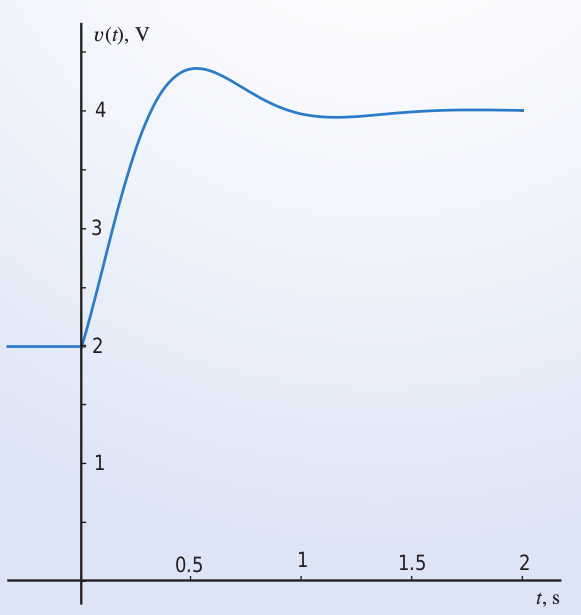
\includegraphics[width=5cm,height=3.5cm]{figura11.png}	
		\end{center}	
		\end{column}
		
	\end{columns}
	
	
\end{tabular}
\end{frame}



% ----------------- NOVA SECÇÂO -----------------------------
\section{Solution of Differential Equations Describing a Circuit (14.6)}
% ----------------- NOVO SLIDE --------------------------------
\begin{frame}[fragile]
	\frametitle{Solution of Differential Equations Describing a Circuit}
\begin{tabular}{ll}

	\begin{columns}
	\small	\begin{column}{1\textwidth}  %%<--- here

	We can solve a set of differential equations describing an electric circuit, using the Laplace transform of
a variable and its derivatives. Here’s the procedure:
	
	
	\small		\begin{enumerate}
\item{Use Kirchhoff’s laws and the element equations to represent the circuit by a differential equation or
set of differential equations.\newline}
\item{Transform each differential equation into an algebraic equation by taking the Laplace transform of
both sides of the equation.\newline}
\item{Solve the algebraic equations to obtain the Laplace transform of the output of the circuit.\newline}
\item{Take the inverse Laplace transform to obtain the circuit output itself.\newline}
					\end{enumerate}				
		\end{column}
	\end{columns}\\
\end{tabular}
\end{frame}
% ----------------- NOVO SLIDE --------------------------------
\begin{frame}[fragile]
	\frametitle{Natural Response of an Overdamped Second-Order Circuit}
\begin{tabular}{ll}
	\begin{columns}
		\begin{column}{1\textwidth}  %%<--- here
		\textbf{EXERCISE 9.4-2} - Find $v_C(t)$ for the circuit shown in Figure below when $i_L(0-)=0.5 \ A$  and $v_C(0-)=2.5 \ V$.

		\begin{center}
    			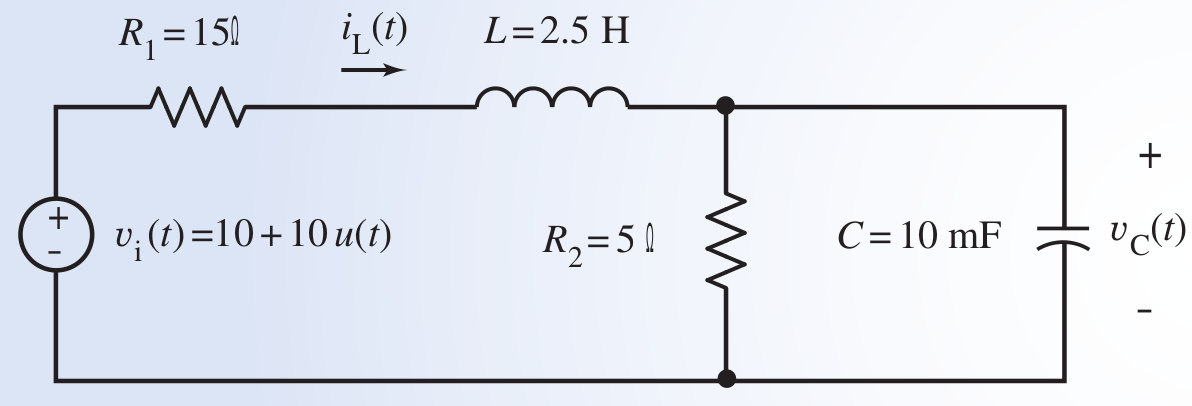
\includegraphics[height=3cm]{figure12.png}	
		\end{center}	
		\scalebox{0.8}{Answer: $v_C(t)=5+4.17e^{-16t}-6.67e^{-10t}\ V$ for t>0}
		\end{column}
	\end{columns}
\end{tabular}
\end{frame}

% ----------------- NOVA SECÇÂO -----------------------------
\section{Circuit Analysis Using Impedance and Initial Conditions (14.7)}
% ----------------- NOVO SLIDE --------------------------------
\begin{frame}[fragile]
	\frametitle{Circuit Analysis Using Impedance and Initial Conditions}
\begin{tabular}{ll}
	\begin{columns}
		\begin{column}{1\textwidth}  %%<--- here
		This method will eliminate the need to write differential equations
to represent the circuit.
		\end{column}
	\end{columns}\\
		\begin{columns}
		\begin{column}{.3\textwidth}  %%<--- here
\center		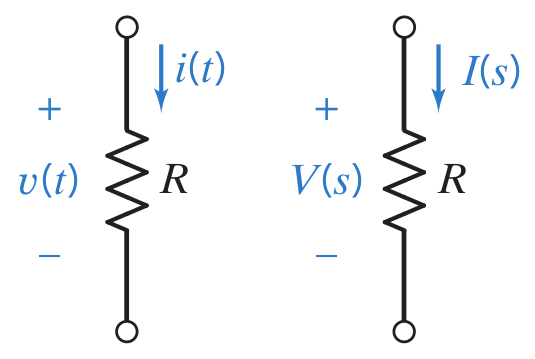
\includegraphics[width=3cm,height=2.5cm]{figure13.png}	
		\end{column}
		\begin{column}{.4\textwidth}  %%<--- here
\center		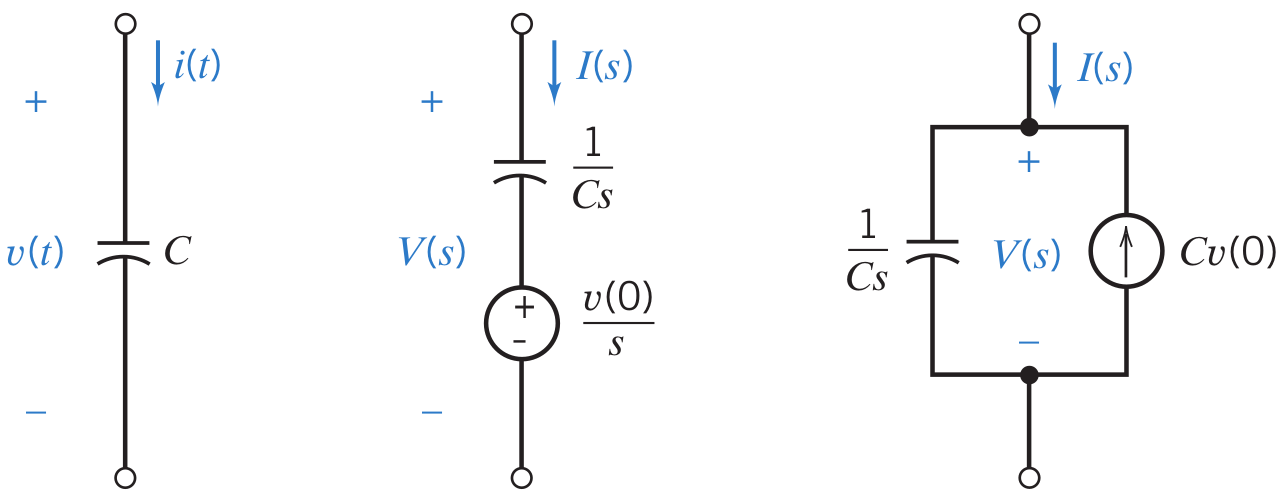
\includegraphics[width=4.5cm,height=2.5cm]{figure14.png}	
		\end{column}
		\begin{column}{.4\textwidth}  %%<--- here
\center		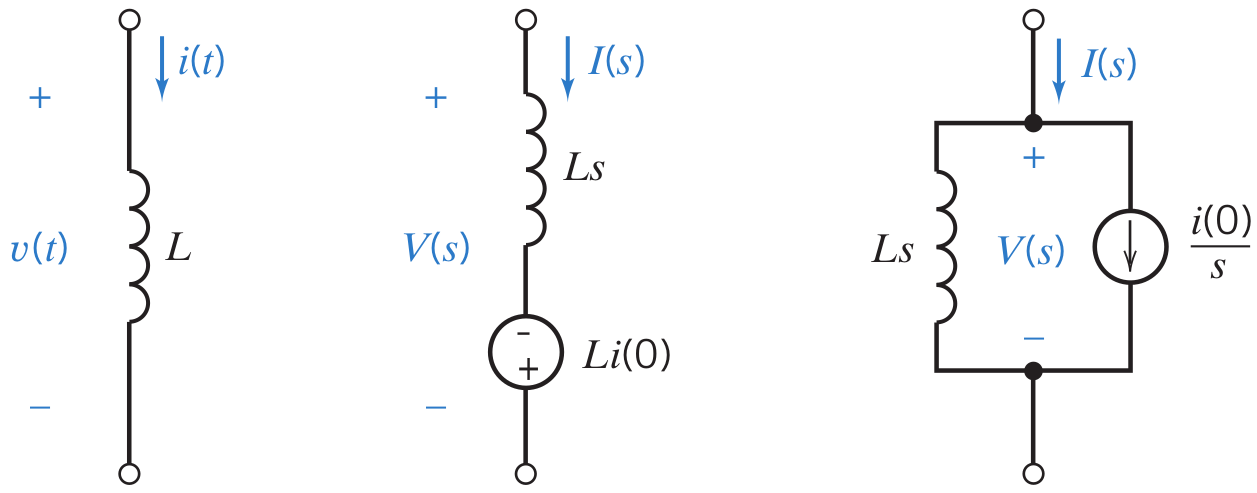
\includegraphics[width=4.5cm,height=2.5cm]{figure15.png}	
		\end{column}
	\end{columns}\\
			\begin{columns}
\footnotesize		\begin{column}{.3\textwidth}  %%<--- here
 \begin{equation}
\begin{aligned}
  v(t)  &= i(t)R\\
  V(s) &= I(s)R \nonumber\\
    Z_R(s) &= \dfrac{V(s)}{I(s)}=R \nonumber\\
  \end{aligned}
\end{equation}	
		\end{column}
\footnotesize		\begin{column}{.4\textwidth}  %%<--- here
\begin{equation}
\begin{aligned}
 v(t) &= \dfrac{1}{C}\int_{0}^{t} i(\tau){d\tau} + v(0)\\
 V(s) &= \dfrac{1}{sC}I(s)+\dfrac{v(0)}{s} \nonumber\\
    Z_C(s) &= \dfrac{V(s)}{I(s)}= \dfrac{1}{sC} \nonumber\\
  \end{aligned}
\end{equation}	
		\end{column}
\footnotesize		\begin{column}{.4\textwidth}  %%<--- here
\begin{equation}
\begin{aligned}
 v(t) &= L\dfrac{d}{dt}i(t)\\
 V(s) &= LsI(s)-Li(0) \nonumber\\
    Z_L(s) &= \dfrac{V(s)}{I(s)}= sL \nonumber\\
  \end{aligned}
\end{equation}		
		\end{column}
	\end{columns}\\
\end{tabular}	
\end{frame}
% ----------------- NOVO SLIDE --------------------------------
\begin{frame}[fragile]
	\frametitle{Circuit Analysis Using the Laplace Transform}
\begin{tabular}{ll}
\footnotesize	\begin{columns}
		\begin{column}{1\textwidth}  %%<--- here
		\textbf{EXAMPLE 14.7-1} - Consider the circuit shown in Figure below. 
		The input to the circuit is the voltage of the voltage source 24 V.
The output of this circuit, the voltage across the capacitor, is given by. $$v_o(t)=16-12e^{-0.6t} \ V \ when t>0$$
Determine the value of the capacitance C.
		\end{column}
		\end{columns}\\
\footnotesize	\begin{columns}
		\begin{column}{.5\textwidth}  %%<--- here
\center		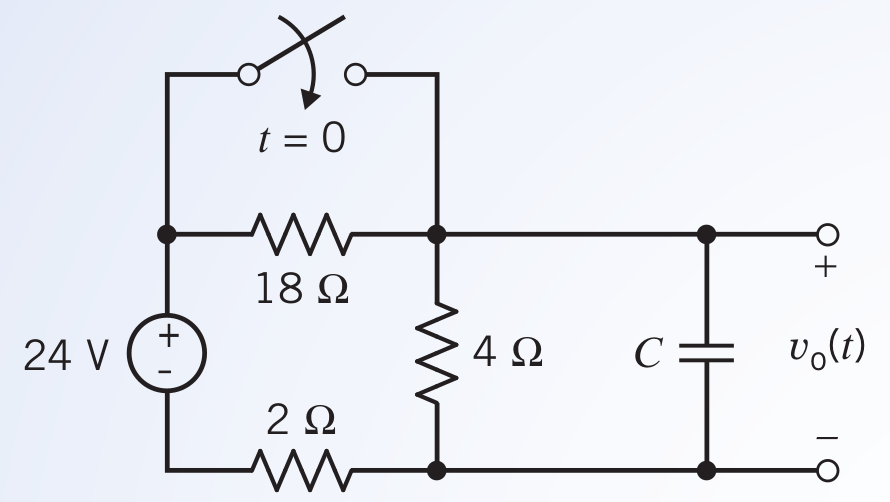
\includegraphics[width=4.5cm,height=2.5cm]{figure16.png}
		\end{column}
		\begin{column}{.5\textwidth}  %%<--- here
\center		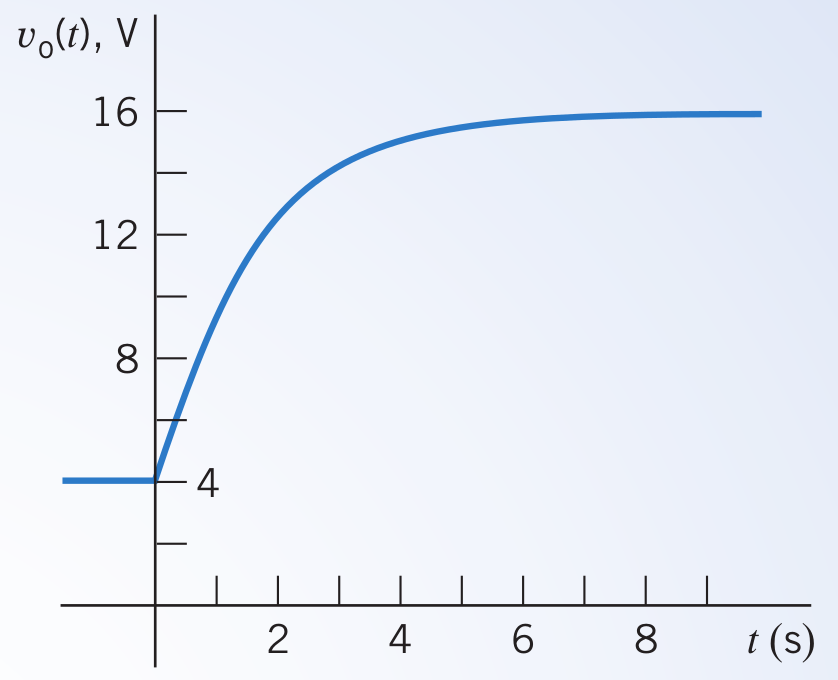
\includegraphics[width=4.5cm,height=2.5cm]{figure17.png}
		\end{column}
	\end{columns}\\
\newline \\ \scalebox{0.8}{Answer: $C=1.25 \ F$}
\end{tabular}
\end{frame}
% ----------------- NOVO SLIDE --------------------------------
\begin{frame}[fragile]
	\frametitle{Circuit Analysis Using the Laplace Transform}
\begin{tabular}{ll}
\footnotesize	\begin{columns}
		\begin{column}{1\textwidth}  %%<--- here
		\textbf{EXAMPLE 14.7-2} - Consider the circuit shown in Figure below. The input to the circuit is
the voltage of the voltage source, 24 V. The output of this circuit, the
voltage across the $6 \Omega$ resistor, is given by. $$v_o(t)=12-6e^{-3.5t} \ V \ when t>0$$
Determine the value of the inductance $L$ and of the resistances $R_1$ and $R_2$ .
		\end{column}
		\end{columns}\\
\footnotesize	\begin{columns}
		\begin{column}{1\textwidth}  %%<--- here
\center		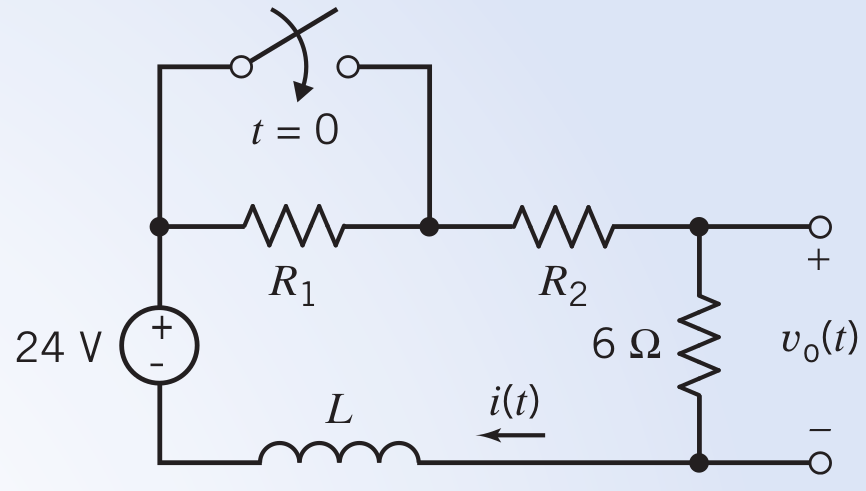
\includegraphics[width=4.5cm,height=2.5cm]{figure18.png}
		\end{column}

	\end{columns}\\
\newline \\ \scalebox{0.8}{Answer: $L=34.29 \ H, \ R_1=12 \ \Omega \, and \ R_2=6\  \Omega.$}
\end{tabular}
\end{frame}
% ----------------- NOVO SLIDE --------------------------------
\begin{frame}[fragile]
	\frametitle{Circuit Analysis Using the Laplace Transform}
\begin{tabular}{ll}
\footnotesize	\begin{columns}
		\begin{column}{1\textwidth}  %%<--- here
		\textbf{EXAMPLE 14.7-3} - Consider the circuit shown in Figure below. 
		The input to the circuit is the voltage of the voltage source 12 V.
The output of this circuit is the current in the inductor $i_L(t)$. Determine the current in the inductor $i_L(t)$, for t > 0.
		\end{column}
		\end{columns}\\
\footnotesize	\begin{columns}
		\begin{column}{1\textwidth}  %%<--- here
\center		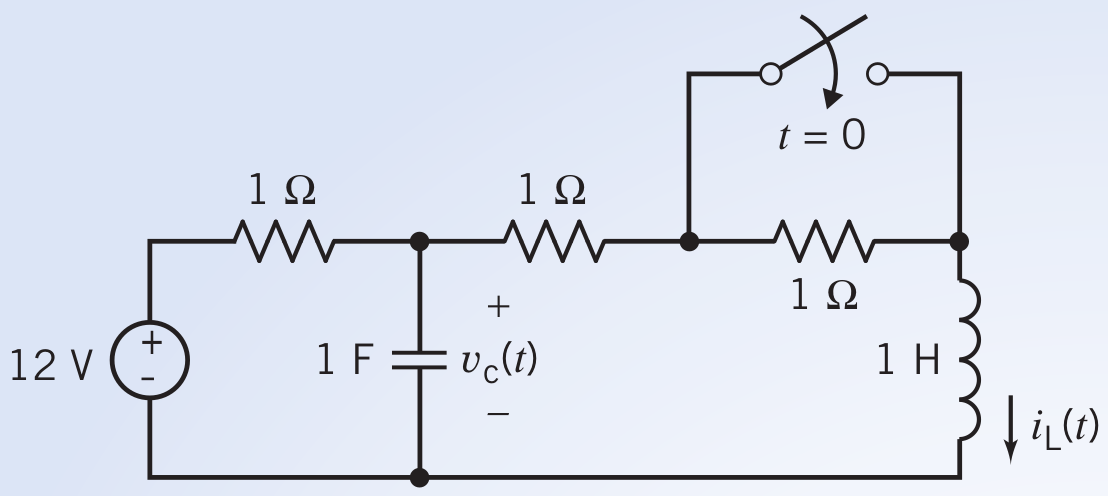
\includegraphics[height=3.cm]{figure19.png}
		\end{column}

	\end{columns}\\
\newline \\ \scalebox{0.8}{Answer: $i_L(t)=6+2\sqrt{2}e^{-t} \sin(t-45^o) \ A \ for \ t>0$}
\end{tabular}
\end{frame}
% ----------------- NOVO SLIDE --------------------------------
\begin{frame}[fragile]
	\frametitle{Circuit Analysis Using the Laplace Transform}
\begin{tabular}{ll}
\footnotesize	\begin{columns}
		\begin{column}{1\textwidth}  %%<--- here
		\textbf{EXAMPLE 14.7-4} - The switch in the circuit shown in Figure below
		closes at time $t=0$. Determine the voltage $v(t)$ after the switch closes.
		\end{column}
		\end{columns}\\
\footnotesize	\begin{columns}
		\begin{column}{1\textwidth}  %%<--- here
\center		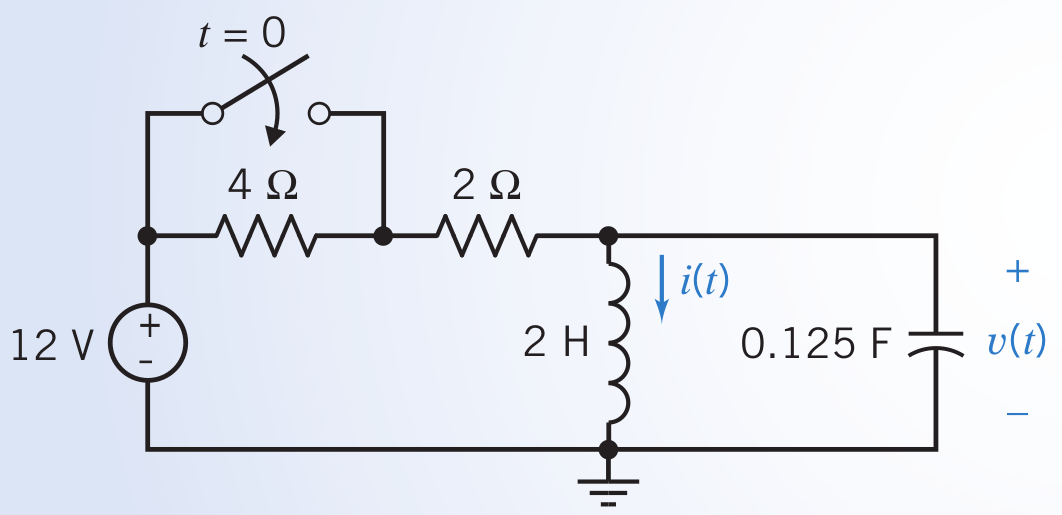
\includegraphics[height=3.5cm]{figure20.png}
		\end{column}

	\end{columns}\\
\newline \\ \scalebox{0.8}{Answer: $v(t)=\mathscr{L}^{-1}\{\dfrac{32}{(s+2)^2}\}=32te^{-2t}u(t) \ V \ for \ t>0$}
\end{tabular}
\end{frame}
% ----------------- NOVA SECÇÂO -----------------------------
\section{Transfer Function and Impedance (14.8)}
% ----------------- NOVO SLIDE --------------------------------
\begin{frame}[fragile]
	\frametitle{Transfer Function and Impedance}
\begin{tabular}{ll}
	\begin{columns}
\footnotesize			\begin{column}{1\textwidth}  %%<--- here
The \textbf{transfer function} of a circuit is defined as the ratio of the Laplace transform of the
response of the circuit to the Laplace transform of the input to the circuit when the initial
conditions are zero.
		\end{column}
		\end{columns}\\
		\begin{columns}
\footnotesize		\begin{column}{0.5\textwidth}  %%<--- here
\newline \newline For the circuit in Figure, the input is the voltage source voltage $v_i(t)$, and the response is the
resistor voltage $v_o(t)$. The transfer function of this circuit, denoted by $H(s)$, is then expressed as
$$H(s)=\dfrac{V_o(s)}{V_i(s)} \ or  \ V_o(s)=H(s)V_i(s)$$
provided all initial conditions are equal to zero. In this case, the only initial condition is the inductor
current, so we require $i(0)=0$.
		\end{column}
		\begin{column}{0.5\textwidth}  %%<--- here
\center		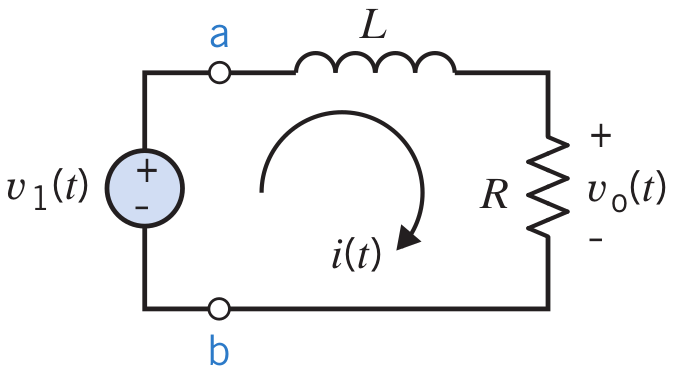
\includegraphics[height=2.2 cm]{figure21.png}
\center		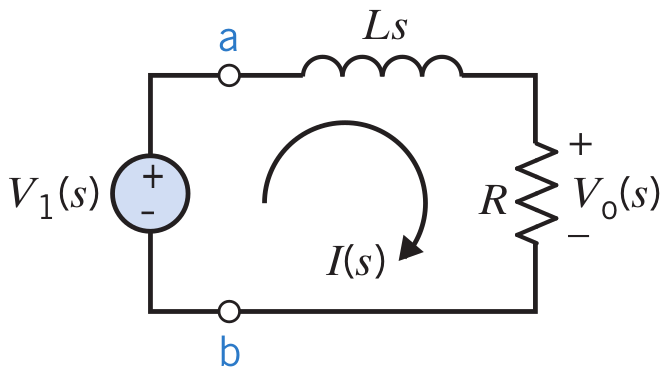
\includegraphics[height=2.2 cm]{figure22.png}
		\end{column}
	\end{columns}\\
\end{tabular}
\end{frame}
% ----------------- NOVO SLIDE --------------------------------
\begin{frame}[fragile]
	\frametitle{Circuit Analysis Using the Laplace Transform}
\begin{tabular}{ll}
\footnotesize	\begin{columns}
		\begin{column}{1\textwidth}  %%<--- here
		\textbf{EXAMPLE 14.8-1} - The input to the circuit shown in Figure below is the voltage $v_i(t)$, 
		and the output is the voltage $v_o(t)$. Determine the
step response of the circuit shown in Figure below.
		\end{column}
		\end{columns}\\
\footnotesize	\begin{columns}
		\begin{column}{1\textwidth}  %%<--- here
\center		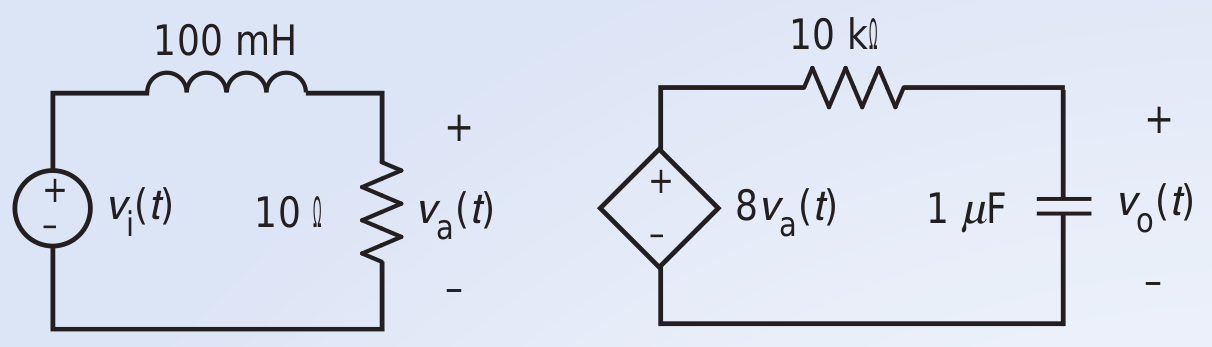
\includegraphics[height=3.5cm]{figure23.png}
		\end{column}

	\end{columns}\\
\newline \\ \scalebox{0.8}{Answer: $v(t)=[8-8(1+100t)e^{-100t}]u(t)$}
\end{tabular}
\end{frame}
% ----------------- NOVO SLIDE --------------------------------
\begin{frame}[fragile]
	\frametitle{Circuit Analysis Using the Laplace Transform}
\begin{tabular}{ll}
\footnotesize	\begin{columns}
		\begin{column}{1\textwidth}  %%<--- here
		\textbf{EXAMPLE 14.8-2} - The input to the circuit shown in Figure below is the voltage $v_i(t)$, 
		and the output is the voltage $v_o(t)$. Design the
circuit shown to have the step response $$v_o(t)=[4-e^{-2t}(4 \cos(4t)-2 \sin(4t))]u(t)$$
		\end{column}
		\end{columns}\\
\footnotesize	\begin{columns}
		\begin{column}{.5\textwidth}  %%<--- here
\center		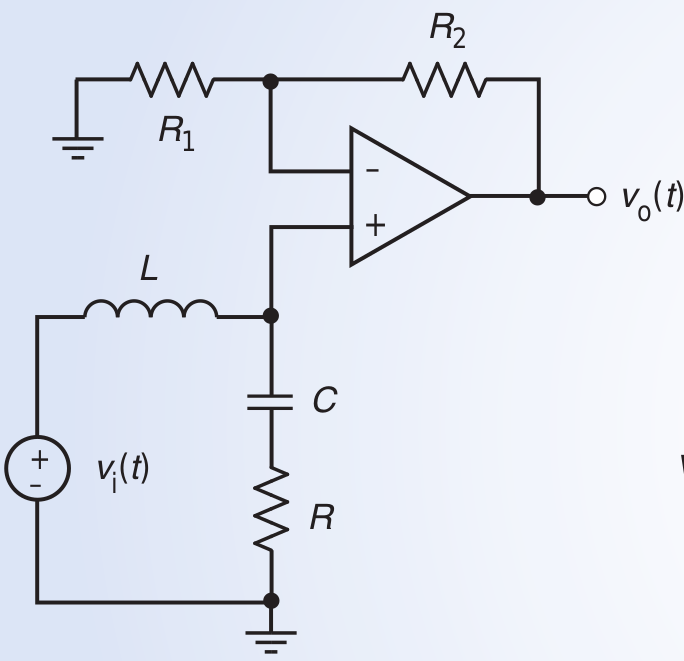
\includegraphics[height=3.5cm]{figure24.png}
		\end{column}
		\begin{column}{.5\textwidth}  %%<--- here
\scalebox{0.8}{Answer: $L=0.5 \ H, C=0.1 \ F, R = 2 \ \Omega, R_1=10k \ \Omega,$}
 \scalebox{0.8}{$ and\ R_2= 30k \ \Omega.$}
		\end{column}
	\end{columns}\\

\end{tabular}
\end{frame}
% ----------------- NOVO SLIDE --------------------------------
\begin{frame}[fragile]
	\frametitle{Circuit Analysis Using the Laplace Transform}
\begin{tabular}{ll}
\footnotesize	\begin{columns}
		\begin{column}{1\textwidth}  %%<--- here
		\textbf{EXAMPLE 14.8-3} - The input to the circuit shown in Figure below is the voltage $v_i(t)$, 
		and the output is the voltage $v_o(t)$. Design the
circuit shown to have the step response $$v_o(t)=[1-(10^4t+1)e^{-10000t}]u(t) \ V$$
		\end{column}
		\end{columns}\\
\footnotesize	\begin{columns}
		\begin{column}{.5\textwidth}  %%<--- here
\center		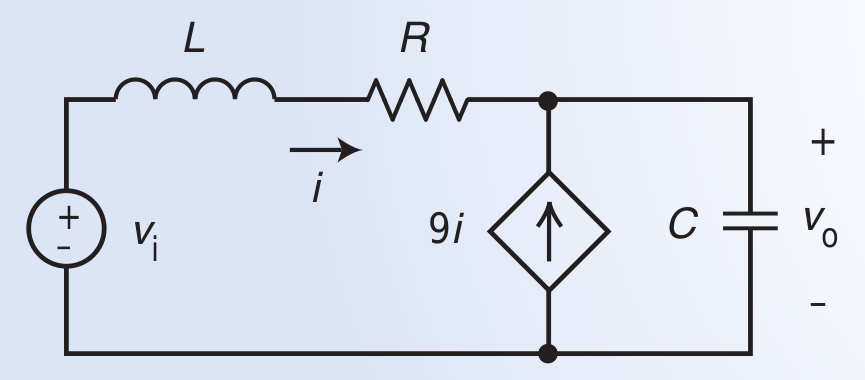
\includegraphics[height=2.5cm]{figure25.png}
		\end{column}
		\begin{column}{.5\textwidth}  %%<--- here
\scalebox{0.8}{Answer: $ R = 200 \ \Omega, \ L=10 \ mH, and \ C=10 \ \mu F$}

		\end{column}
	\end{columns}\\

\end{tabular}
\end{frame}
% ----------------- NOVA SECÇÂO -----------------------------
\section{Convolution (14.9)}
% ----------------- NOVO SLIDE --------------------------------
\begin{frame}[fragile]
	\frametitle{Convolution}
\begin{tabular}{ll}

	\begin{columns}
\footnotesize		\begin{column}{0.5\textwidth}  %%<--- here
In this section, we consider the problem of determining the response of a
linear, time-invariant circuit to an arbitrary input, $x(t)$.
	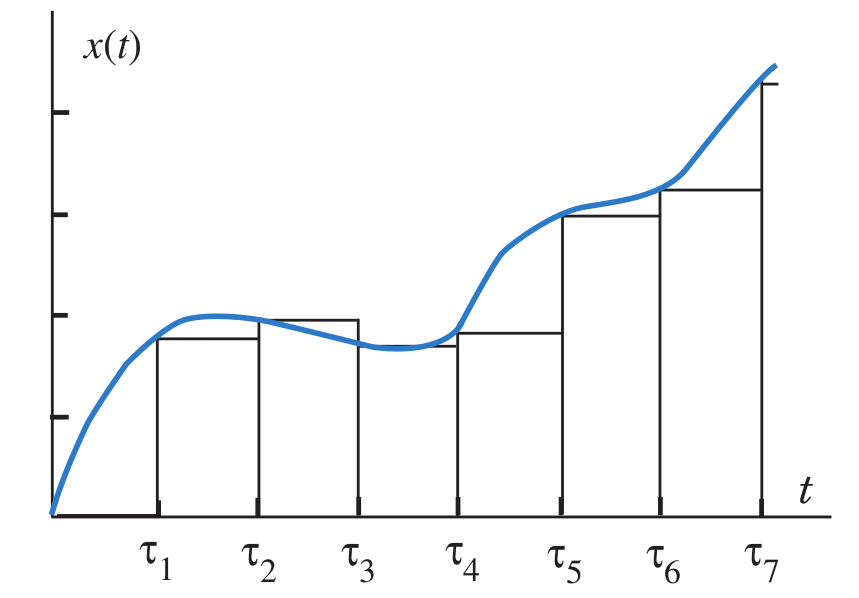
\includegraphics[height=3cm]{figure26.png} \\

Consider:
$$
	    \delta_\Delta(t)=
	    \begin{cases}
	    \dfrac{1}{\Delta}, \ when \ 0 \leq  t < \Delta \\
	    0, \  otherwise \\
	    
	    \end{cases}
	    $$

	    
		\end{column}
\scriptsize		\begin{column}{0.5\textwidth}  %%<--- here
Thus, \\		
		$x(\Delta)=x(\tau_1)=x(\Delta)\delta_\Delta(t-\Delta) \Delta$\\
		$x(k\Delta)=x(\tau_k)=x(k\Delta)\delta_\Delta(t-k\Delta) \Delta$\\
		$\hat{x}(t)=\sum_{k=-\infty}^{\infty}x(k\Delta)\delta_\Delta(t-k\Delta) \Delta$\\
		$x(t)=\lim_{\Delta \to 0}\sum_{k=-\infty}^{\infty}x(k\Delta)\delta_\Delta(t-k\Delta) \Delta$\\
			$$x(t)=\int_{-\infty}^{\infty} x(\tau) \delta(t-\tau) d\tau $$
How \newline 	
		$x(t) \rightarrow y(t), \  kx(t) \rightarrow ky(t) \ or \  k\delta(t-t_0) \rightarrow kh(t-t_0)$ \newline  \\ 
We have \\		
		$x(k\Delta)=x(k\Delta)\delta_\Delta(t-k\Delta) \Delta$\\
		$y(k\Delta)=x(k\Delta)h_\Delta(t-k\Delta) \Delta$\\
		$y(t)=\lim_{\Delta \to 0}\sum_{k=-\infty}^{\infty}x(k\Delta)h_\Delta(t-k\Delta) \Delta$\\
		$$y(t)=\int_{-\infty}^{\infty} x(\tau) h(t-\tau) d\tau $$
		\end{column}
	\end{columns}\\	
\end{tabular}	
\end{frame}
% ----------------- NOVA SECÇÂO -----------------------------
\section{Stability (14.10)}
% ----------------- NOVO SLIDE --------------------------------
\begin{frame}[fragile]
	\frametitle{Stability}
\begin{tabular}{ll}

	\begin{columns}
\footnotesize		\begin{column}{0.5\textwidth}  %%<--- here
A circuit is said to be \textbf{stable} when the response to a bounded input signal is a bounded output
signal. A circuit that is not stable is said to be \textbf{unstable}. \newline \\


Consider a circuit represented by the transfer function H(s). Factoring the denominator of the
transfer function gives

$$H(s)=\dfrac{N(s)}{(s-p_1)(s-p_2)....(s-p_n)}$$

The $p_i$ are the poles of the transfer function, also called the poles of the circuit. \newline \\

\textbf{A circuit is stable if, and only if, all of its poles have negative real parts.}
		\end{column}
\scriptsize		\begin{column}{0.5\textwidth}  %%<--- here
We can also use the impulse response $h(t)$ to determine whether a circuit is stable.

		$$\arrowvert y(t) \arrowvert=\arrowvert \int_{-\infty}^{\infty} x(\tau) h(t-\tau) d\tau \arrowvert$$
		$$\arrowvert y(t) \arrowvert=\arrowvert \int_{-\infty}^{\infty} h(\tau) x(t-\tau) d\tau \arrowvert$$
		$$\arrowvert y(t) \arrowvert \leq  \int_{-\infty}^{\infty} \arrowvert h(\tau)\arrowvert \arrowvert x(t-\tau)\arrowvert d\tau $$
If \ 
$\arrowvert x(t-\tau)\arrowvert  \leq B$
$$\arrowvert y(t) \arrowvert \leq B \int_{-\infty}^{\infty} \arrowvert h(\tau)\arrowvert  d\tau $$
Thus, a circuit is said to be \textbf{stable} when 
$$\int_{-\infty}^{\infty} \arrowvert h(\tau)\arrowvert  d\tau \leq \infty$$
		
		\end{column}
	\end{columns}\\	
\end{tabular}
\end{frame}

\end{document} 

